\subsection{Programa final Unity PRO}

A partir del programa utilizado para los primeros registros, se realizó modificaciones necesarias para borrar y agregar variables que se creyeron necesarias a la hora de implementar el proyecto.


\subsubsection{Direcciones utilizadas}
\fcolorbox{red}{yellow}{Las direcciones utilizadas para unity + ifix ponerlo despues de SCADA?}


\subsection{Adquisición de datos}
Para realizar la estimación de la planta del sistema se utilizó el protocolo OPC en conjunto con Matlab. Por medio de OFS (OPC Factory Server, software de Schneider), se procedió a crear y configurar un servidor con la dirección correspondiente y se seleccionó el programa realizado en UnityPro donde se encontraban las variables necesarias (Figura \ref{fig:opc1}).

\begin{figure}[htbp]
	\centering
	\subfigure[]{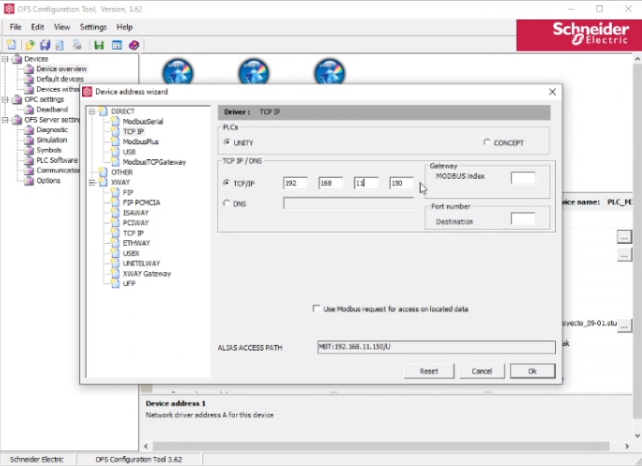
\includegraphics[width=70mm]{ofs1.png}}
	\subfigure[]{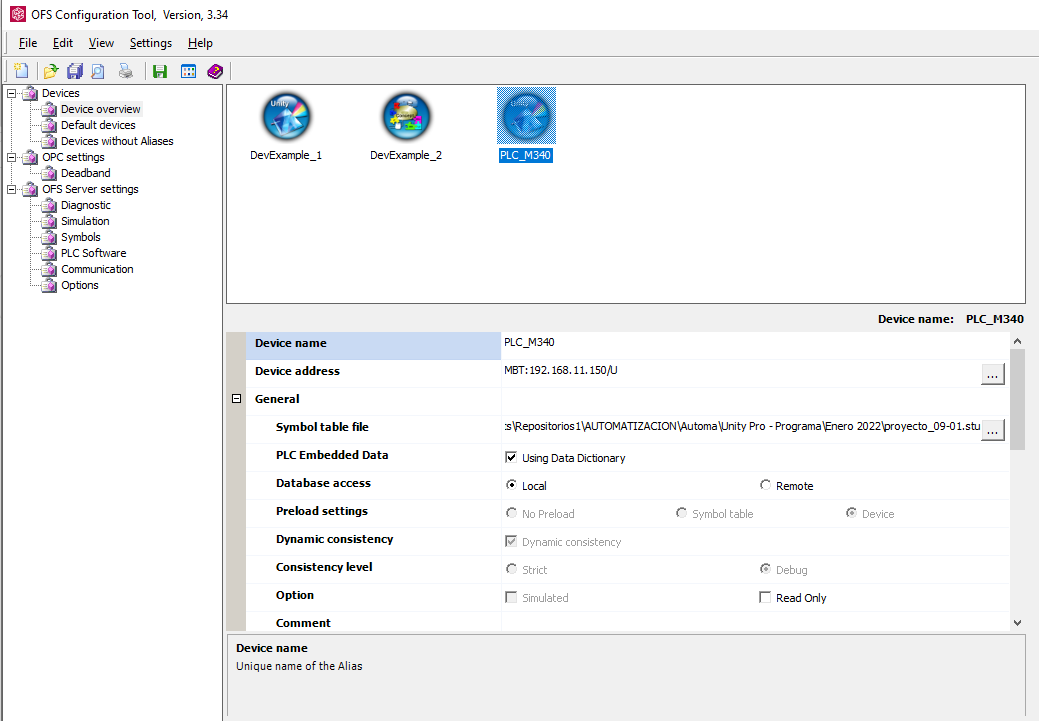
\includegraphics[width=70mm]{ofs2.png}}
	\caption{Configuración OPC} \label{fig:opc1}
\end{figure}


Una vez configurado el servidor se abre el programa \textbf{OPC Factory Server} dando inicio al servidor (Figura \ref{fig:opc2}a). Para observar si la comunicación esta establecida de forma correcta, se utilizó el programa \textbf{OFS Client} dónde se debió agregar el tag correspondiente a la variable a observar (Figura \ref{fig:opc2}b)

\begin{figure}[htbp]
	\centering
	\subfigure[OPC Factory Server]{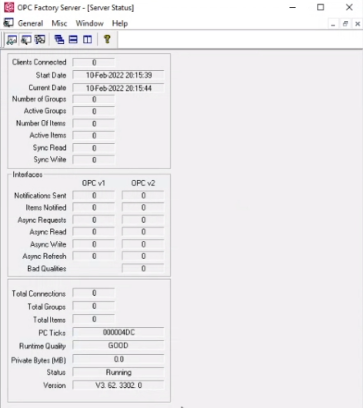
\includegraphics[width=40mm]{ofs3.png}}
	\subfigure[OFS Client]{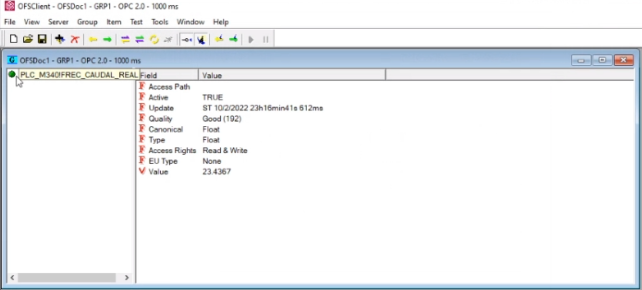
\includegraphics[width=80mm]{ofs4.png}}
	\caption{Conexión servidor OPC} \label{fig:opc2}
\end{figure}

Una vez corroborada la comunicación con el servidor OPC, se procedió a crear un cliente OPC en Simulink (perteneciente a Matlab) para adquirir y guardar las variables necesarias. 


\subsubsection{Uso de Matlab}
En el entorno Simulink se procedió a configurar un bloque de cliente OPC con la dirección IP donde se encuentra el servidor previamente creado. Luego, para leer las variables necesarias se creó un bloque de lectura OPC (Figura \ref{fig:opcsimu} a) y con un bloque \textit{Scope}, se activó la opción para que se guarden los vectores de las variables a estudiar (Figura \ref{fig:opcsimu} b). 


\begin{figure}[htbp]
	\centering
	\subfigure[]{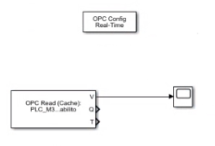
\includegraphics[width=40mm]{ofs5.png}}
	\subfigure[]{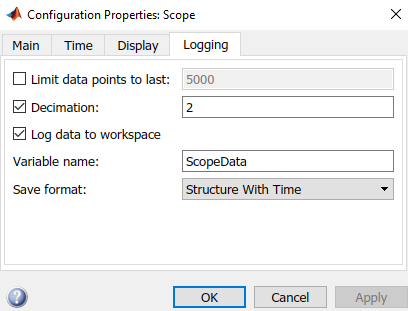
\includegraphics[width=60mm]{ofs6.png}}
	\caption{Cliente OPC en Simulink} \label{fig:opcsimu}
\end{figure}



\subsubsection{Estimación de la planta}

Para realizar la estimación de las plantas se utilizó el método matemático de sistema de primer orden con retardo (Figura \ref{fig:1erorden}), cuya función de transferencia es: \\
\begin{equation}
	G(s)\;=\;\frac K{1\;+\;\tau\;.\;s}e^{-T.s}
\end{equation}


Dónde:
\begin{itemize}
	\item K:  Ganancia del sistema $K = \frac{\triangle y}{\triangle u}$
	\item $\tau$: constante de tiempo
	\item T= Retardo
\end{itemize}

Los valores correspondientes de cada elemento para cada planta son los siguientes: 
\fcolorbox{red}{yellow}{los saque de lectura\_csv\_vs\_mod y de cvs drive}
\begin{table}[]
	\centering
	\begin{tabular}{llll}
		& PIT001 & PIT002 & FT001 \\
		Ay & 1.4208 & 13.29 & 4.18 \\
		Au & 200 & 200 & 300 \\
		T & 0.6 & 1.1 &  \\
		\textbackslash{}tau & 1.7 & 2 & 
	\end{tabular}
\end{table}


\begin{figure}[htb]
	\centering
	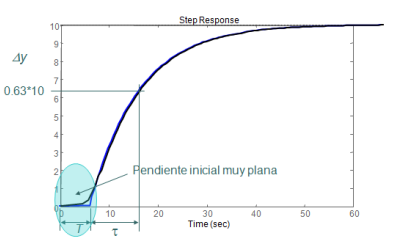
\includegraphics[scale=1]{1erorden.png}
	\captionof{figure}{Placa con sensores}
	\label{fig:1erorden}
\end{figure}


\subsubsection{PID calculado}
Cada PID se calculó con \fcolorbox{red}{yellow}{Tune PID controllers}, se buscó que las respuestas sean \fcolorbox{red}{yellow}{críticamente amortiguado}, los valores recomendados son:
\begin{table}[]
	\centering
	\begin{tabular}{llll}
		& PIT001 & PIT002 & FT001 \\
		Kp & ??? & ??? & ??? \\
		Ki & ??? & ??? & ??? \\
		Kd & ??? & ??? & ??? \\
	\end{tabular}
\end{table}

Se puede observar que el controlador PID es del tipo proporcional integrador, se realizó de esta forma ya que la ganancia en los diferentes escalones en la planta no era constante. Al utilizar un PI genera una salida con error de estado estacionario cero. 


\fcolorbox{red}{yellow}{Estuve viendo las curvas con escalones donde se ve que la ganancia estática se modifica frente a diferentes escalones. Si el objetivo fuese calcular un controlador para ese sistema una buena opción seria un controlador PI. De esta forma, la acción integral va a tratar de hacer que el error de estado estacionario sea cero frente a una entrada escalón. Además, los problemas que pueden existir en el envejecimiento de componentes, errores en el modelado y variaciones en la ganancia estática se van a mitigar con la parte integral del controlador. Obviamente al cambiar la planta la respuesta va a cambiar pero se va a cumplir la consigna de seguir la referencia. Para mostrar esto es posible calcular un controlador para un sistema y luego probar el controlador en los dos sistemas. Eso hice en el pdf que les adjunto con un sistema con 3 polos reales. Más detalles pueden encontrar en el libro de Ogata o Control avanzado de Karl Astrom, capitulo 3.
De esta forma, me da la sensación que para los objetivos de esta materia plantear un controlador PI para un controlador me parece bien.}


